\documentclass{beamer}


\usepackage[utf8]{inputenc}
\usepackage{amsmath}
\usepackage{amsfonts}
\usepackage{amssymb}
\usepackage{graphicx}
\usepackage{ragged2e}  % `\justifying` text
\usepackage{booktabs}  % Tables
\usepackage{tabularx}
\usepackage{tikz}      % Diagrams
\usetikzlibrary{calc, shapes, backgrounds}
\usepackage{amsmath}
\usepackage{amssymb}
\usepackage{dsfont}
\usepackage{url}       % `\url
\usepackage{listings}  % Code listings
\usepackage[T1]{fontenc}
\usepackage[percent]{overpic}
\usetikzlibrary{trees}

\usepackage{theme/beamerthemehbrs}

\author[MAS]{Hassan Umari}
\title{Introduction to ROS}
\subtitle{Foundation Course}
\institute[HBRS]{Hochschule Bonn-Rhein-Sieg}
\date{\today}
\subject{ROS workshop}

% \thirdpartylogo{path/to/your/image}


\begin{document}
{
\begin{frame}
\titlepage
\end{frame}
}


\section{What is ROS?}


\subsection{What ROS is}
\begin{frame}{What ROS is}
\framesubtitle{Robot Operating System}
    \begin{itemize}
        \item Short for: Robot Operating System.
        \item A collection of libraries and tools.
        \item It helps software developers create robot
        applications. 
    \end{itemize}
\end{frame}



\begin{frame}[plain]{}
    \centering
    \includegraphics[width=.66\linewidth]{figures/stop_reinventing_theWheel.jpg}
    
\tiny{http://www.willowgarage.com/blog/2010/04/27/reinventing-wheel}
\end{frame}


\begin{frame}{What ROS is}
    \framesubtitle{Robot Operating System}
    \begin{itemize}
        \item A way to standardize writing software for robots.
        \item It enhances {\huge code reusability} \includegraphics[scale=0.02]{figures/recycling.png}.
        \item ROS is open-source \includegraphics[scale=0.09]{figures/open_source.png}.
        \item It is a meta-operating system.
        \item ROS can be installed on Ubuntu and Debian (so it’s currently supported on Linux only).
        
        \includegraphics[width=.1\linewidth]{figures/linux_logo.png}
        \includegraphics[width=.1\linewidth]{figures/ubuntu_logo.png} 
        \includegraphics[width=.06\linewidth]{figures/debian_logo.png} 
    \end{itemize}
\end{frame}


\subsection{What ROS is NOT}
\begin{frame}{What ROS is NOT}
    \framesubtitle{Robot Operating System}
    \begin{itemize}
        \item It is NOT a programming language.
        \item It is NOT an integrated development environment
        (IDE).
        \item It is NOT a stand-alone operating system 
    \end{itemize}
\end{frame}


%---------------------------

\section{Analogy Between ROS and Operating Systems}

\begin{frame}{Analogy Between ROS and Operating Systems}
    \begin{overpic}[width=.45\linewidth]{figures/analogy1.png}
        \put (130,80) {Software Applications}
        \put (130,50) {work on}
        \put (130,20) {Different hardware}        
    \end{overpic}
\end{frame}

\begin{frame}{Analogy Between ROS and Operating Systems}
    \centering
    \begin{overpic}[width=.4\linewidth]{figures/analogy2.png}
        \put (35,90) {Application} 
        \put (9,65) {\footnotesize Operating System} 
        \put (12,43) {\footnotesize Device Drivers}   
    \end{overpic}
\end{frame}

\begin{frame}{Analogy Between ROS and Operating Systems}
    \centering
    \begin{overpic}[width=.3\linewidth]{figures/analogy3.png}
        \put (2,102) {Mapping algorithm}
        \put (21.5,74) {ROS} 
        \put (11,49) {Laser driver} 
        \put (-25,10) {Laser scanner} 
    \end{overpic}
\end{frame}


\begin{frame}{Analogy Between ROS and Operating Systems}
    \centering
    \begin{overpic}[width=.8\linewidth]{figures/analogy4.png}
        \put (34,72) {Mapping algorithm}
        \put (46.5,54) {ROS}
        \put (2.3,29) {Laser driver}
        \put (38,29) {Laser driver}
        \put (75,29) {Laser driver}
    \end{overpic}
\end{frame}

\begin{frame}{Analogy Between ROS and Operating Systems}
    \begin{overpic}[width=.8\linewidth]{figures/analogy4.png}
        \put (34,72) {Mapping algorithm}
        \put (46.5,54) {ROS}
        \put (2.3,29) {Laser driver}
        \put (38,29) {Laser driver}
        \put (75,29) {Laser driver}
    \end{overpic}
\end{frame}

\begin{frame}{Analogy Between ROS and Operating Systems}
    \begin{overpic}[width=.8\linewidth]{figures/analogy5.png}
        \put (34,72) {Mapping algorithm}
        \put (46.5,54) {ROS}
        \put (2.3,29) {Laser driver}
        \put (38,29) {Laser driver}
        \put (75,29) {Laser driver}
        \put (105,10) {\footnotesize Different hardware}
    \end{overpic}
\end{frame}

\begin{frame}{Analogy Between ROS and Operating Systems}
    \begin{overpic}[width=.8\linewidth]{figures/analogy6.png}
        \put (34,72) {Mapping algorithm}
        \put (46.5,54) {ROS}
        \put (2.3,29) {Laser driver}
        \put (38,29) {Laser driver}
        \put (75,29) {Laser driver}
        \put (105,10) {\footnotesize Different hardware}
        \put (105,30) {\footnotesize Different drivers}
    \end{overpic}
\end{frame}

\begin{frame}{Analogy Between ROS and Operating Systems}
    \begin{overpic}[width=.8\linewidth]{figures/analogy7.png}
        \put (34,72) {Mapping algorithm}
        \put (46.5,54) {ROS}
        \put (2.3,29) {Laser driver}
        \put (38,29) {Laser driver}
        \put (75,29) {Laser driver}
        \put (105,10) {\footnotesize Different hardware}
        \put (105,30) {\footnotesize Different drivers}        
        \put (105,58) {\footnotesize Data received in}
        \put (105,54) {\footnotesize the same message}
        \put (105,50) {\footnotesize format}
    \end{overpic}
\end{frame}

\begin{frame}{Analogy Between ROS and Operating Systems}
    \begin{overpic}[width=.8\linewidth]{figures/analogy7.png}
        \put (34,72) {Mapping algorithm}
        \put (46.5,54) {ROS}
        \put (2.3,29) {Laser driver}
        \put (38,29) {Laser driver}
        \put (75,29) {Laser driver}
        \put (105,10) {\footnotesize Different hardware}
        \put (105,30) {\footnotesize Different drivers}        
        \put (105,58) {\footnotesize Data received in}
        \put (105,54) {\footnotesize the same message}
        \put (105,50) {\footnotesize format}
        \put (105,72) {\footnotesize No change}
    \end{overpic}
\end{frame}

\begin{frame}{Analogy Between ROS and Operating Systems}
    \begin{overpic}[width=.45\linewidth]{figures/analogy8.png}
        \put (130,77) {Robot Applications}
        \put (3,75) {\scriptsize Mapping}
        \put (33,75) {\scriptsize Navigation}
        \put (66,75) {\scriptsize pick \& place}
        \put (130,50) {work on}
        \put (130,20) {Different hardware}        
    \end{overpic}
\end{frame}

\begin{frame}[label=figs2]{Analogy Between ROS and Operating Systems}
\centering
 \scalebox{0.9}{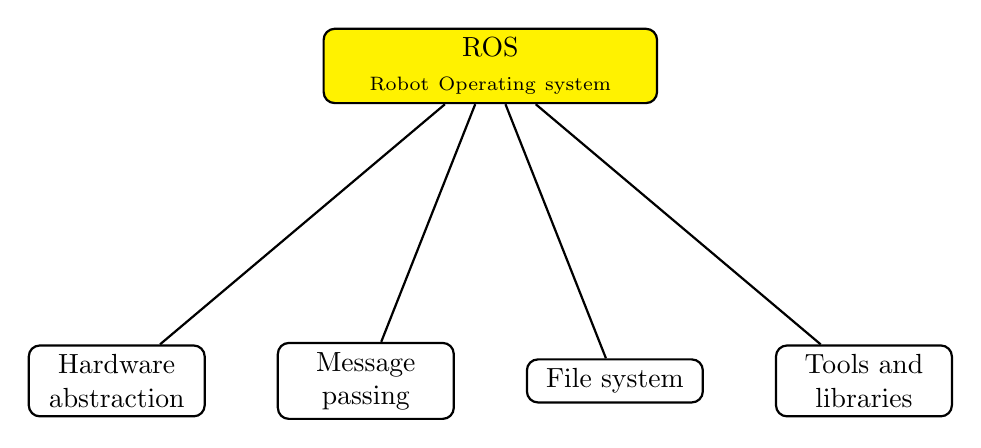
\begin{tikzpicture}[sibling distance=9em, level distance = 4.0cm, thick,
every node/.style = {shape=rectangle, rounded corners,
    draw, align=center}]]
\node [text width=4cm, fill = yellow]{ROS \\ \scriptsize Robot Operating system}
child { node [text width=2cm]{Hardware abstraction} }
child { node [text width=2cm]{Message passing} }
child { node [text width=2cm]{File system} }
child { node [text width=2cm]{Tools and libraries} };
\end{tikzpicture}}
\end{frame}





%---------------------------

\section{Features of ROS}

\begin{frame}{Features of ROS}

\begin{itemize}
        \item Language independent.
        \item Distributed and Modular.
        \item A lot of libraries and tools.
        \item Open Source.
        \item Active Community.
\end{itemize}
\end{frame}

\subsection{Language independent}
\begin{frame}{Features of ROS}
\framesubtitle{Language independent}    
\begin{itemize}
    \item ROS functionalities are implemented as a library in different programming languages.
    \item  These libraries are referred to as ROS client libraries.
\end{itemize}
\end{frame}

\begin{frame}{Language independent}
    \framesubtitle{Features of ROS}    

    ROS client libraries.  
    
    \vspace{0.5cm}
    \centering
\scalebox{0.8}{%
  \begin{minipage}{\textwidth}
    \begin{itemize}
        \item Main ROS Client libraries:
        \begin{itemize}
            \item roscpp \hspace{7cm} \includegraphics[width=.06\linewidth]{figures/cpp_logo.png}
            \item rospy  \hspace{7.1cm} \includegraphics[width=.08\linewidth]{figures/python_logo.png}
            \item roslisp \hspace{7cm} \includegraphics[width=.06\linewidth]{figures/lisp_logo.png}
        \end{itemize}
        \item Experimental ROS client libraries:
        \begin{itemize}
            \item rosjava \hspace{7cm} \includegraphics[width=.06\linewidth]{figures/java_logo.png}
            \item rosruby \hspace{7cm} \includegraphics[width=.06\linewidth]{figures/ruby_logo.png}
            \item and some others..
        \end{itemize}
        \item ROS support on MATLAB:
        \begin{itemize}
            \item Robotics System Toolbox \hspace{4.3cm} \includegraphics[width=.06\linewidth]{figures/matlab_logo.png}
        \end{itemize}
    \end{itemize}
\end{minipage}%
}
\end{frame}


\subsection{Distributed and Modular}

\begin{frame}{Distributed and Modular}
    \framesubtitle{Features of ROS}    
    \begin{itemize}
        \item ROS supports running processes on multiple computers connected together through a LAN.
        \item In a system running ROS, there will be multiple of processes where each process can do
        certain task. A process can be changed without altering the remaining processes.
    \end{itemize}
\end{frame}


\subsection{A lot of libraries and tools}

\begin{frame}{A lot of libraries and tools}
    \framesubtitle{Features of ROS}    
    \begin{itemize}
        \item Examples of libraries:
            \begin{itemize}
                \item Navigation stack.
                \item SLAM (gmapping, hector SLAM, etc..).
                \item Localization (amcl, etc..).
                \item Motion planning for manipulators (MoveIt)
                \item Support for popular libraries (OpenCV, PCL).
            \end{itemize}
            
        \item Examples of tools:
            \begin{itemize}
                \item RVIZ:3D Visualization.
                \item ROS bag files: Logging Sensor Data.
                \item Catkin: A Build System.
                \item Command line tools.
            \end{itemize}        
    \end{itemize}
\end{frame}


\subsection{Bad Things About ROS}

\begin{frame}{Bad Things About ROS}
            \begin{itemize}
                \item Learning ROS needs time. 
                \item It needs a computer. Does not work on a microcontroller!
                \item Not optimized for multiple robots.
                \item Supported only on Linux, no support for Windows or macOS.
            \end{itemize}  
\end{frame}





%---------------------------

\section{ROS Concepts}

\begin{frame}{ROS Concepts}
\tikzstyle{every node}=[draw=white,thick,anchor=west]
\tikzstyle{selected}=[draw=red,fill=red!30]
\tikzstyle{optional}=[dashed,fill=gray!50]
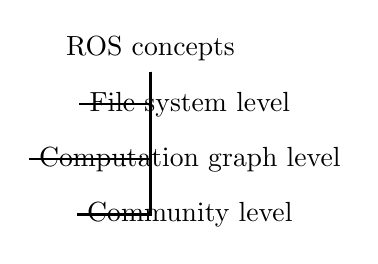
\begin{tikzpicture}[%
thick, grow via three points={one child at (0.5,-0.7) and
    two children at (0.5,-0.7) and (0.5,-1.4)},
edge from parent path={(\tikzparentnode.south) |- (\tikzchildnode.west)}]
\node {ROS concepts}
child { node {File system level}}		
child { node {Computation graph level}}
child { node {Community level}};
\end{tikzpicture}
\end{frame}


\subsection{File system level}

\begin{frame}{File system level}
  \framesubtitle{ROS Concepts}
    
 \centering
 \scalebox{0.9}{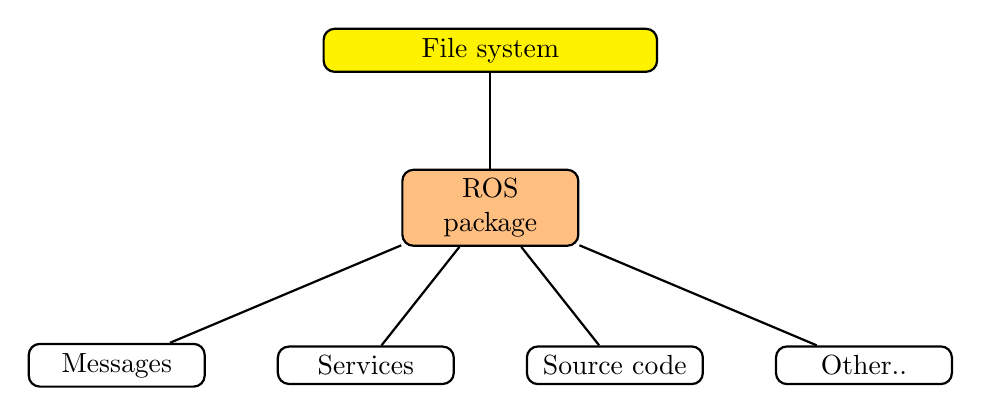
\begin{tikzpicture}[sibling distance=9em, level distance = 2.0cm, thick,
     every node/.style = {shape=rectangle, rounded corners,
         draw, align=center}]]
        \node [text width=4cm, fill = yellow]{File system}
         child { node [text width=2cm, fill = orange!50]{ROS package} 
        child { node [text width=2cm]{Messages} }
        child { node [text width=2cm]{Services} }
        child { node [text width=2cm]{Source code} }
        child { node [text width=2cm]{Other..} }
        };
        \end{tikzpicture}}
\end{frame}


\begin{frame}{File system level}
    \framesubtitle{ROS Concepts}
    
    \centering
    \scalebox{0.9}{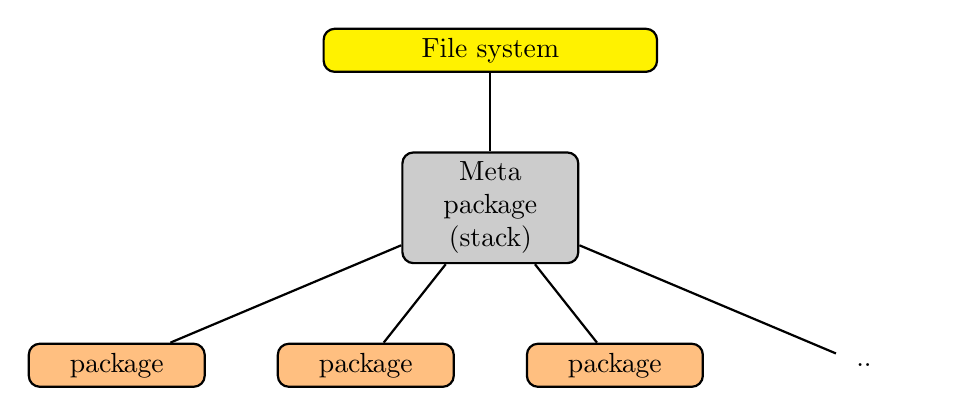
\begin{tikzpicture}[sibling distance=9em, level distance = 2.0cm, thick,
        every node/.style = {shape=rectangle, rounded corners,
            draw, align=center}]]
        \node [text width=4cm, fill = yellow]{File system}
        child { node [text width=2cm, fill = black!20]{Meta package \\ (stack)} 
            child { node [text width=2cm, fill = orange!50]{package} }
            child { node [text width=2cm, fill = orange!50]{package} }
            child { node [text width=2cm, fill = orange!50]{package} }
            child { node [text width=2cm, fill = none, draw = none]{..} }
        };
        \end{tikzpicture}}
\end{frame}


\begin{frame}{File system level}
    \framesubtitle{ROS Concepts}
Inside a ROS package:

\vspace{0.5cm}
\centering
\includegraphics[width=.9\linewidth]{figures/example_package.png}
\end{frame}

    
\subsection{Computation graph level}

\begin{frame}{Computation graph level}
    \framesubtitle{ROS Concepts}
\end{frame}



\subsection{Community level}

\end{document}
